\documentclass[11pt]{article}
\usepackage{tikz}
%\usepackage{xfrac}
%\usepackage{hyperref}
%\usepackage[export]{adjustbox}
\def\checkmark{\tikz\fill[scale=0.4](0,.35) -- (.25,0) -- (1,.7) -- (.25,.15) -- cycle;} 
\usepackage{proj} 	% pull in style header
\usepackage{array}
\usepackage{sectsty}
\usepackage{soul}
\usepackage{float}
\restylefloat{table}

\lhead{ECE544: Embedded Systems on FPGAs}


%----------------------------------------------------------------------------------------
%	TITLE SECTION
%----------------------------------------------------------------------------------------


\newcommand{\horrule}[1]{\rule{\linewidth}{#1}} % Create horizontal rule command with 1 argument of height

\title{	
\normalfont \normalsize 
\textsc{\LARGE Portland State University}\\[1.5cm] % Name of your university/college
\textsc{\Large Embedded Systems on FPGAs}\\[0.5cm] % Major heading such as course name
\textsc{\large ECE544}\\[0.5cm] % Minor heading such as course title
%\textsc{Portland State University} \\ [25pt] % Your university, school and/or department name(s)
\horrule{1.2pt} \\[0.4cm] % Thin top horizontal rule
\huge Closed-Loop Control With PWM \\ % The assignment title
\horrule{1.2pt} \\[0.5cm] % Thick bottom horizontal rule
}

%----------------------------------------------------------------------------------------
%	AUTHOR SECTION
%----------------------------------------------------------------------------------------


\begin{document}\raggedright
\author{Erik Rhodes \and Caren Zgheib} % Your name
\maketitle % Print the title
\thispagestyle{empty}
\cfoot{\textit{Page \thepage { of} \pageref{LastPage}}}
\lhead{ECE544}
\chead{Project 2}
\rhead{Erik Rhodes \& Caren Zgheib}


\begin{figure}[h]\centering
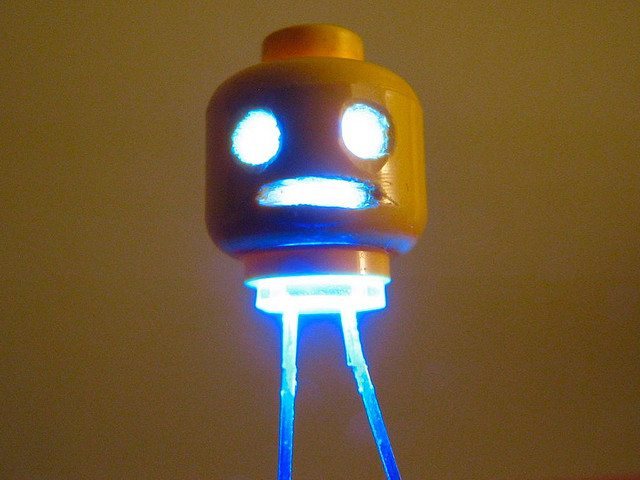
\includegraphics[height=0.65\textwidth]{images/LED_halloween.jpg}
	%\caption{Gameplay Block Diagram}
		\label{LED}
	\end{figure}
	
\newpage

% -------------------------PROJECT DELIVERABLES -----------------------------------
%A five to seven (5 to 7) page project report explaining the operation of your design, most notably your control algorithms and user interface (if it is noticeably different than what I suggested).  Please include at least one “interesting” graph showing the results from each of the control algorithms.  Each graph should be labeled with the control parameters you used to make the run. I’d like to see a characterization graph for your control system, as well. This graph should show circuit output response vs. control input. Please list the work done by each partner. Be sure to note any work that you borrowed from somebody else (other than me). I’d also like an estimate of how long you spent on the project and what problems you had to overcome.

%Source code for your C application(s). Please “take ownership” of your application.  I want to see your program structure and comments, not mine. Your system.mhs, system.mss and system.ucf files.  All files regarding your new peripheral for the light sensor, including the Verilog hardware, and driver code.
% ----------------------------------------------------------------------------------


%TODO Tasks: Pictures: diagram of our system (in progress), Serial chart graph results of each test. 
% Code snippets needed: driver code, scaling, pushbutton logic


%Caren: You really won't have to mess with much formatting or Tex language here. 
%If for right now you just want to edit in vim or notepad thats fine, you just can't test anything out.  At some point before our next project you should download the Latex software package.  
% It's pretty easy to see how things work, but I'll give you a few useful ones:
% \textbf{example} bolds and \texttt{example} makes them a different font
% to put in quotes, use ``these''
% \section{} and \subsection{} should be pretty self explanatory
% pictures, tables, etc should have labels  than can be referred to in other parts of the document (with \ref{name_of_label}). Just look at the things I did.
% My friend put together a presentation you could look at for reference
% https://github.com/ekrause/LaTeX-Presentation 


\section{Introduction} 
This project demonstrates how closed-loop control can be used in modern applications.  Our embedded system monitored the brightness of an LED with a light sensor and calculated the corresponding PWM output to stabilize the brightness at the desired setpoint.

	\begin{figure}[h]\centering
	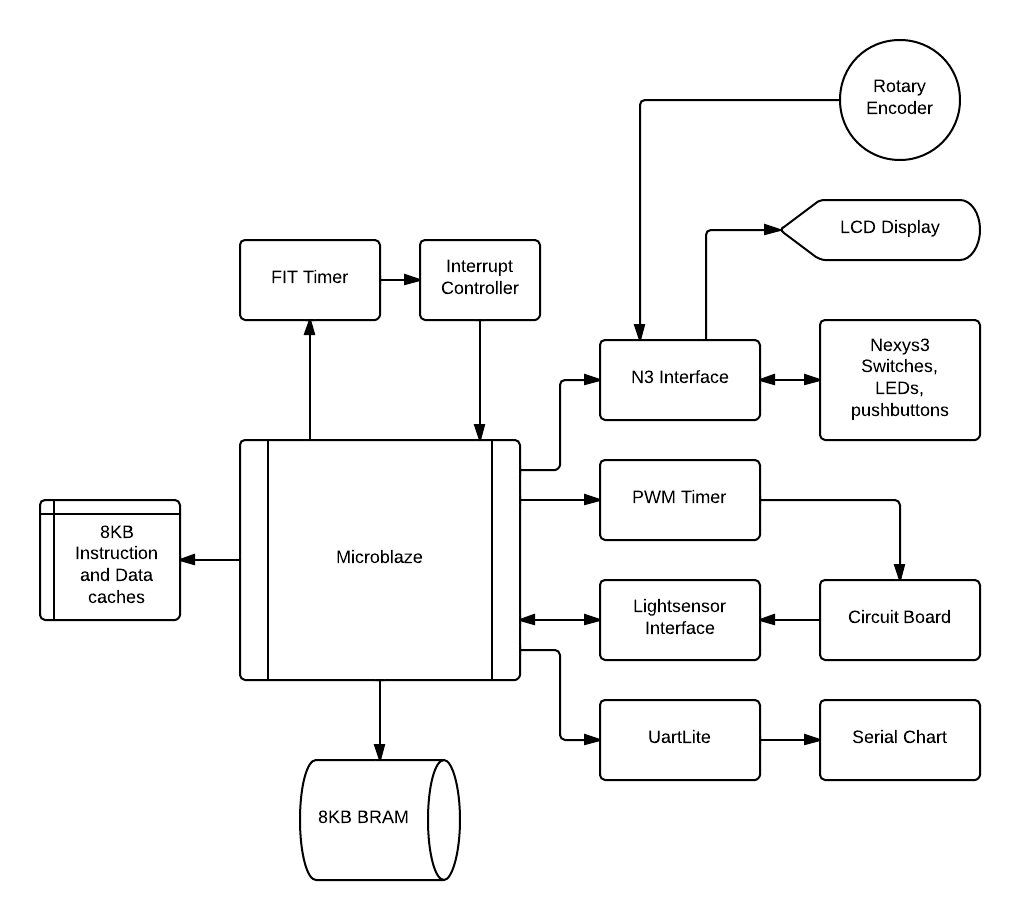
\includegraphics[height=0.7\textwidth]{images/block_diagram.png}
	\caption{Block Diagram of Control System}
		\label{diagram}
	\end{figure}


\section{System Design}
%TODO Reference
As seen in figure \ref{diagram}, our embedded system includes numerous peripherals and components. 
 Our \textbf{lightsensor} peripheral interacts with the circuit we built on a breadboard.  This connects the \textbf{PWM timer} to the LED (through pin 7), and receives the detected brightness from the light sensor through another pin (pin 9).  The \textbf{Uartlite} peripheral sends the computed data to the external hardware serially through a USB port.  This data can then be seen using different programs, such as \emph{Putty} or \emph{Serial Charter}.  The graphs showing our results (reference) were created using \emph{Serial Charter}. The \textbf{N3EIF} interface controls the communication to the LCD display and the rotary encoder. In order to allow this functionality, 8KB of \textbf{BRAM} was added, and instruction and data caches were included as well.  While GPIO pins were technically included in our system, they existed simply for debugging purposes and therefore were not added to the diagram.


\section{Implementation}

\subsection{Control Methodology}
Being able to control a dynamic system is an integral part of many everyday systems.  Accomplishing this requires a feedback loop with an external measurement of the output being fed back into the system.  These systems can be controlled in a number of ways.  Two popular methods are \textbf{Bang Bang} and \textbf{PID}.   

\subsubsection{Bang Bang} 
Bang bang is quite straightforward: if the output is lower than desired, the controller puts the control signal at its highest amount.  Likewise, if the output is higher than desired, the signal is set to the lowest level.  While sometimes effective, this is a crude and cheap method for controlling systems, and is usually only used in devices where accuracy is not extremely important. The algorithm used in our program is seen below.

\vspace{12pt}

 \begin{lstlisting}[caption=Bang Bang Algorithm, label=bang]		
 	 for (smpl_idx = 1; smpl_idx < NUM_FRQ_SAMPLES; smpl_idx++)
 	    {
 	        sample[smpl_idx] = LIGHTSENSOR_Capture(LIGHTSENSOR_BASEADDR, slope, offset, is_scaled, freq_min_cnt);
 	        volt_out = (-3.3 / 4095.0) * (sample[smpl_idx]) + 3.3; 
 	        if (volt_out < setpoint)
 	        {
 	            Status = PWM_SetParams(&PWMTimerInst, pwm_freq, MAX_DUTY);
 	            delay_msecs(1);
 	            if (Status == XST_SUCCESS)
 	            {
 	                PWM_Start(&PWMTimerInst);
 	            }
 	        }
 	        else
 	        {
 	            Status = PWM_SetParams(&PWMTimerInst, pwm_freq, MIN_DUTY);
 	            delay_msecs(1);
 	            if (Status == XST_SUCCESS)
 	            {
 	                PWM_Start(&PWMTimerInst);
 	            }
 	        }
 	        delay_msecs(100);
 	    }
  \end{lstlisting}

\subsubsection{PID}
The more prevalent method, PID, involves making multiple calculations to predict the accurately control the behavior of the output.  The proportional (P) method involves using the previous error margin to calculate the next appropriate one.  The integral (I) method calculates how the system behaves over time, and the derivative (D) calculates how fast the output is changing at that point in time.  Our implementation is seen in listing \ref{PID}. \\
Using a specific arrangement of these parameters will yield a large increase in accuracy, so tuning the application is desirable.  When tuning, we first attempted to follow the \emph{Ziegler-Nichols} method.  After understanding how each method changes the output, we modified the parameters as we saw fit to acquire the most accurate configuration for our control system. 

\vspace{12pt}

 \begin{lstlisting}[caption=PID Algorithm, label=PID]		
     for (smpl_idx = 1; smpl_idx < NUM_FRQ_SAMPLES; smpl_idx++)
     {
         delay_msecs(100);
 
         // get count from light sensor and convert to voltage 
         sample[smpl_idx] = LIGHTSENSOR_Capture(LIGHTSENSOR_BASEADDR, slope, offset, is_scaled, freq_min_cnt);
         volt_out = (-3.3 / 4095.0) * (sample[smpl_idx]) + 3.3;

         // calculate derivative;
         error = setpoint - volt_out;
         deriv = error - prev_error;
 
         // calculate integral
         if (error < setpoint/10) integral += error;
         else integral = 0; 
 
         // Control offset is gotten from characterization
         volt_out = offset + (error * prop_gain) + (deriv * deriv_gain) + (integral * integral_gain);
         duty_out = (volt_out)* (MAX_DUTY+1)/VOLT_MAX;
 
         // establish bounds
         if (duty_out < 1) duty_out = 1;
         if (duty_out > 99)duty_out = 99;
 
         // activate PWM
         Status = PWM_SetParams(&PWMTimerInst, pwm_freq, duty_out);
         if (Status == XST_SUCCESS)	 PWM_Start(&PWMTimerInst);
     } 
  \end{lstlisting}
  
  


\subsection{Peripheral Interface}
The \textbf{TSL237} light-to-frequency converter outputs a period that directly corresponds to the intensity of the light emitted from the LED.  The PWM detection module receives this information and converts it to a ``count'', which is then scaled to fit within the parameters (between 0 and 4095) needed for our control calculations.  These functions are handled in the light sensor driver.  The driver initially converted the scaled counts to a voltage, but we later decided to move that functionality to the program application.
The peripheral has the user-visible registers described in table \ref{registers}.

	\begin {table}[H]
	\begin {center} 
	\vspace{15pt}
	
	\begin{tabular}{||c|c|c|c||}\hline
		\textbf{Register}	&	\textbf{Number}	&	\textbf{Format} 	& 	\textbf{Description}		\\\hline
		Control				&	slv\_reg0		&	{RESERVED[30:0], EN} &  Enable of the peripheral 		\\\hline
		Status				&	slv\_reg1		&	{RESERVED[30:0], EN} & Current settings of the peripheral		\\\hline
		HighTime			&	slv\_reg2		&    HighTime[31:0] 	&	Detected high time count  			\\\hline
		Period				&	slv\_reg3		&  	Period[31:0] 		&	Detected period count 			\\\hline
		SpareReg1			&	slv\_reg4		&	RESERVED[31:0] 		& 	No specific purpose 			\\\hline
		SpareReg2			&	slv\_reg5		&	RESERVED[31:0] 		& 	No specific purpose 			\\\hline
	\end{tabular}
		\caption {Lightsensor peripheral registers} \label{registers}
	\end{center}
	\end{table} 
	
\subsection{Peripheral Driver}
The \texttt{lightsensor} driver enables the software application to communicate with the external peripheral. It has six functions: 

\begin{itemize}
\item \textbf{LIGHTSENSOR\_Init()} Initializes the \texttt{lightsensor} peripheral driver. It waits until the light sensor self test is done then it sets the control enable bit to 0.
\item \textbf{LIGHTSENSOR\_Start()} Starts the PWM detection in the peripheral. This function sets the Control Enable bit to 1.
\item \textbf{LIGHTSENSOR\_Stop()} Stops the PWM detection in the peripheral. This function sets the Control Enable bit to 0.
\item \textbf{LIGHTSENSOR\_Capture()} This function returns the period count by reading the PERIOD register. If the characterize function has been called already, the \texttt{is\_scaled} boolean would be set to true and the capture function returns the scaled period count based on the formula  
\begin{equation}
count = (Xuint32)(slope * (period - min)+ 1); \nonumber
\end{equation}

\item \textbf{LIGHTSENSOR\_SetScaling()} Not implemented since we decided to do the scaling directly in the application program. Here is what the scaling looks like in the code:
\begin{equation}
diff = freq\_max\_cnt - freq\_min\_cnt; \nonumber
\end{equation}
\begin{equation}
slope = 4095.0 / diff; \nonumber
\end{equation}

\item \textbf{LIGHTSENSOR\_Count2Volts()} Also not used because we do the conversion in the program directly. Here is what the conversion looks like in the code:
\begin{equation}
volt\_out = (-3.3 / 4095.0) * (sample[smpl\_idx]) + 3.3;  \nonumber
\end{equation}
\end{itemize}

%  
% Perhaps a subsubsection about the components to creating the embedded system?
% JC, JD header and ucf file stuff? (no need)
% Picture of breadboard? (no need)

\subsection{Frequency detection}
%TODO Include info about how the detection worked
The measurements output by the light sensor were received by a hardware module that interpreted the data.  This Verilog program closely resembles the PWM detection module done in project 1.  It increments the count on each clock edge, depending on whether the input is high or low.  Once a full period is detected, the high count and period are sent to registers which are able to be read by the light sensor driver.  

\subsection{User Controls} 
The program starts by characterizing the system.  This allows the initial scaling to be performed, which varies by the amount of light detected by the light sensor. After this is done, the default control parameter values are displayed and the user is given a chance to change them.  The type of test and starting input voltage can also be selected.  Once these have been configured, the user starts the test with the rotary button.  When it has finished, long pressing on the rotary button sends the data to the computer connected serially via the UART port.  If the user wants to change the test, they can modify the switch values and update the LCD by pressing on the rotary button.  While the user interface remained close to the recommended specifications, it also included a few features that made it amazingly incredible. The control assignments are seen in table \ref{controls}.
 
 
	\begin {table}[h!]
	\begin {center} 
	\vspace{15pt}
	
	\begin{tabular}{||c|c|c||}\hline	
		\textbf{Name}	&	\textbf{Value}	&	\textbf{Function}		\\\hline
		Switch[1:0]		&	00		&	Bang Bang 		\\\hline
		Switch[1:0]		&	01		&	PID 		\\\hline
		Switch[1:0]		&	10		&	Unused	 	\\\hline
		Switch[1:0]		&	11		&	Characterization 		\\\hline
		Switch[2]		&	0		&	Vin Low		\\\hline
		Switch[2]		&	1		&	Vin High	\\\hline
		Pushbutton		&	North	&	Move Cursor		\\\hline
		Pushbutton		&	East	&	Increase Value		\\\hline
		Pushbutton		&	West	&	Decrease Value		\\\hline
		LCD Display 	&	Row 1	&	PID Values	\\\hline
		LCD Display 	&	Row 2	&	Setpoint and Offset	\\\hline
		Rotary Encoder	& Clockwise	& 	Increase Setpoint		\\\hline
		Rotary Encoder	& Counter-Clockwise	& 	Decrease Setpoint		\\\hline
		Rotary Encoder	& Press Button		& 	Next section \\\hline
		Rotary Encoder	& Long Press Button	& 	Initiate test \\\hline
		
	\end{tabular}
		\caption {Nexys3 Controls} \label{controls}
	\end{center}
	\end{table} 		
  

\section{Results}

%TODO: Include graphs of our characterization and other stuff, with all the variables and the setpoint stuff.  
% Caren: just put your screenshots in the images folder and label them exactly how I've put them below.  Then just put any descriptions and specifications (setpoint, offset, PID values, etc...) and maybe how acceptable they seemed.  I'll take care of the rest.
% From Robin: Please include at least one “interesting” graph showing the results from each of the control algorithms.  Each graph should be labeled with the control parameters you used to make the run. I’d like to see a characterization graph for your control system, as well. This graph should show circuit output response vs. control input.

\subsection{Characterization}
Our characterization is fairly linear. It drops off at the end because the stepping from low to high ends at the 99th sample.

	\begin{figure}[H]\centering
	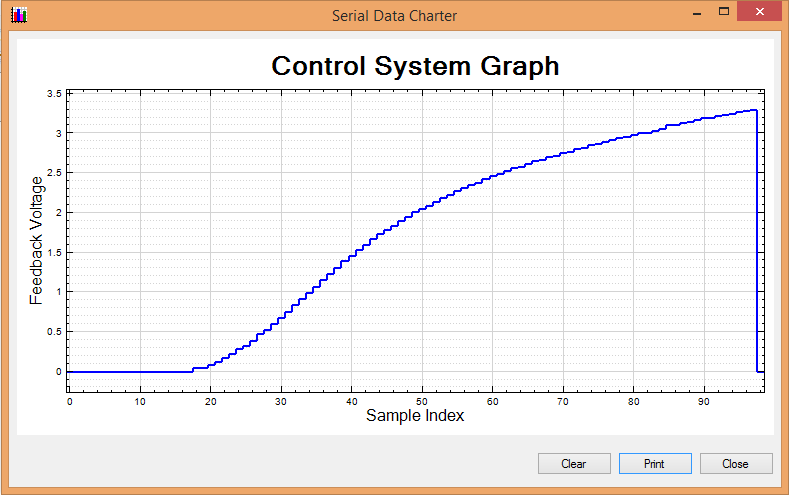
\includegraphics[height=0.7\textwidth]{images/characterize.png}
	\caption{Characterization of light sensor}
		\label{characterization}
	\end{figure}

\subsection{Bang Bang}
Oscillates back and forth around the setpoint. 

	\begin{figure}[H]\centering
	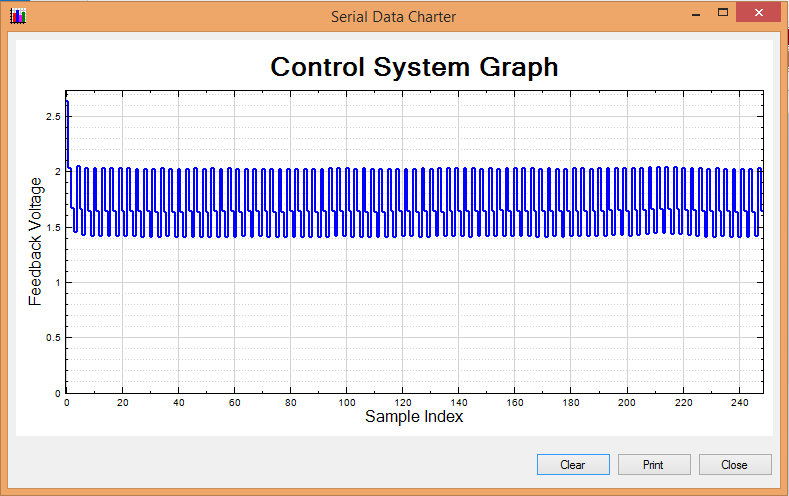
\includegraphics[height=0.7\textwidth]{images/BBh146.png}
	\caption{Results using Bang Bang Control: setpoint=1.46 , starting from Vin high}
		\label{bang_bang_h}
	\end{figure}
	
	\begin{figure}[H]\centering
	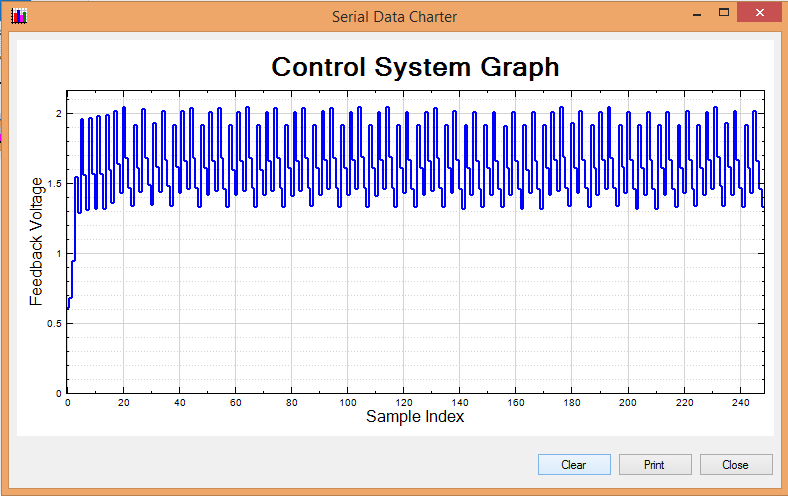
\includegraphics[height=0.7\textwidth]{images/BBl146.png}
	\caption{Results using Bang Bang Control: setpoint=1.46 , starting from Vin low}
		\label{bang_bang_l}
	\end{figure}

	
\subsection{PID}
The following figures show some accurate results:

	\begin{figure}[H]\centering
	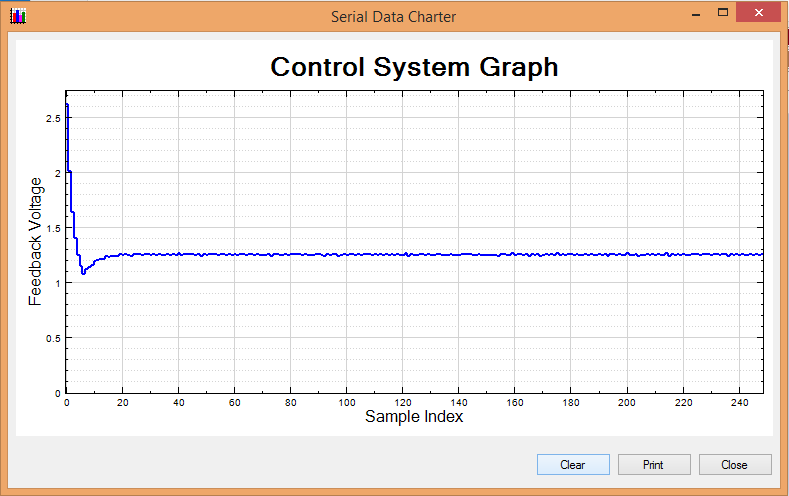
\includegraphics[height=0.7\textwidth]{images/P3-1I1-1D1-2H1-26O2.png}
	\caption{Results using PID Control: P gain = 3.1, I gain = 1.1, D gain = 2.1, Offset = 2 and setpoint = 1.26. (starting from Vin High)}
		\label{PID}
	\end{figure}

	\begin{figure}[H]\centering
	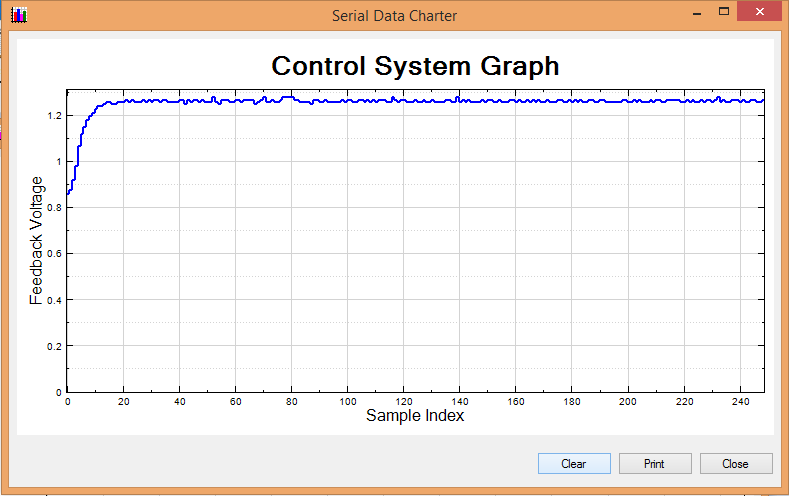
\includegraphics[height=0.7\textwidth]{images/P3-1I1-1D1-2L1-26O2.png}
	\caption{Results using PID Control: P gain = 3.1, I gain = 1.1, D gain = 2.1, Offset = 2 and setpoint = 1.26. (starting from Vin Low)}
		\label{PID2}
	\end{figure}

%	\begin{figure}[h]\centering
%	\includegraphics[height=0.7\textwidth]{images/PID3.png}
%	\caption{Results using PID Control}
%		\label{PID3}
%	\end{figure}

%... not sure how many we need

	
\section{Conclusion}

We split up the project tasks in the following manner:

	%table "Division of Tasks" 
	\begin {table}[H]
	\begin {center} 
	
	\begin{tabular}{||l|c|c|c|c||}\hline	
		\textbf{Task}					& \textbf{Erik} & \textbf{Caren}  				\\\hline
	Peripheral							&	 			&	\checkmark			\\\hline
	Lightsensor Driver					&	 			&	\checkmark			\\\hline
	User application					&	\checkmark	&						\\\hline
	Integration							&	\checkmark	&	\checkmark			\\\hline	
	Documentation						&	\checkmark	&	\checkmark			\\\hline

	
	\end{tabular}
		\caption {Division of Tasks} \label{Division of Tasks}
	\end{center}
	\end{table}
	
	
	\subsection{Challenges}
		
		\begin{itemize}				
		\item \textbf{Tools}: The Xilinx tool chain was quite a hassle to deal with.  There was also a problem connecting one of our circuit boards to the Nexys3.  Additionally, the UART serial USB connection also caused repeated BSOD's on our computer.
		\item \textbf{Hardware interfacing}: Although we took the same module used in project one for the hardware PWM detection, it did not work.  After narrowing down this problem, we swapped the module out and were able to receive reliable results.
		\item \textbf{Typecasting}: In several different places, using the wrong type gave us incorrect values.  Making sure each variable was initialize and cast to the correct type took time, and before this was done we received incorrect or imprecise values.
		\item \textbf{Integration}: We divided the project into two different parts, which were both written in a relatively quick amount of time.  Given the number of components in this system, however, it was quite a challenge to integrate and fix all the different issues that occurred when they were merged together. 
		\end{itemize}

While this project is certainly good practice for the real world, the amount of problems we faced was quite numerous.  It is especially frustrating when the roadblocks we faced were not actually involving our code or the algorithms we were using.  Instead, much of our time was spent wasted on getting the tools to cooperate.  This lead to us spending at least 40 hours each on this project.  With that being said, the concept of closed-loop control was quite interesting, and the results we finally achieved were satisfying. 
	
\end{document}